\section{Controllabilità di un sistema lineare}

\subsection{Problema di controllo}
Introduco la definizione di \emph{problema di controllo}.
Questa si basa sulla definizione~\ref{def:sistema-dinamico} in cui,
assieme allo spazio delle fasi, viene aggiunto uno \emph{spazio dei controlli}.
Di seguito userò la notazione
\begin{equation*}
    \mathcal U^{\mathcal T},\ \text{con } \mathcal T \text{ intervallo}
\end{equation*}
per indicare lo spazio di tutte le funzioni da $\mathcal T$ a $\mathcal U$.

\begin{definition}
    La quadrupla $\left( \Sigma, \mathcal T, \mathcal U, \phi \right)$ in cui:
    \begin{itemize}
        \item $\Sigma$ è uno spazio delle fasi
        \item $\mathcal T$ è un insieme del tempo
        \item $\mathcal U \subseteq \R^n$ è l'insieme dei controlli ammessi
        \item $\phi$ è un applicazione detta \textbf{mappa di transizione} del problema:
            \begin{equation*}
                  \begin{array}{cccc}%
                      \phi: &D_\phi &\to &\Sigma \\
                      &\phi^t(\b x_0,\omega) &\mapsto &\b x(t)
                  \end{array}%
            \end{equation*}
            con $D_\phi$ dato da
            \begin{equation*}
                D_\phi = \left\{(t, \b x, \omega) | t \in \mathcal T, \b x \in \Sigma, \omega \in \mathcal U^{[0, t[ \subseteq \mathcal T} \right\}
            \end{equation*}
    \end{itemize}
    definisce un \textbf{problema di controllo} se e solo se valgono le seguenti proprietà:
    \begin{itemize}
        \item \textbf{Identità:}
            $\phi^0(\b x_0, \omega) = \b x_0$
        \item \textbf{Composizione e restrizione:}
            Se $\phi^t(\b x_0, \omega_1) = \b x_1$ e $\phi^s(\b x_1, \omega_2) = \b x_2$
            allora $\phi^{t+s}(\b x_0, \omega) = \b x_2$, con $\omega = \omega_1 \circ \omega_2$.
            È valido anche il contrario, ovvero, se $\phi^{t+s}(\b x_0, \omega) = \b x_2$, posso
            scrivere $\omega = \omega_1 \circ \omega_2$ per cui vale $\phi^t(\b x_0, \omega_1) = \b x_1$ e $\phi^s(\b x_1, \omega_2) = \b x_2$.
        \item \textbf{Non-trivialità:}
            Per ogni stato $\b x \in \Sigma$ esiste sempre un tempo $t$ e un
            controllo $\omega$ per cui $(t, \b x, \omega) \in D_\phi$
    \end{itemize}
    \label{def:problema-di-controllo}
\end{definition}
\todo{Questa definizione l'ho presa dal sontag e ho cercato di alleggerire appena la notazione, rendendola simile
alla definizione di sistema dinamico. Il concetto alla base è lo stesso, spero che vada bene lo stesso.}

Per descrivere un problema di controllo, posso usare un'equazione del moto con la stessa forma
della~\eqref{eq:sistema-non-lineare}:
\begin{equation*}
    \dot {\b x} = \b a(\b x, \b u),\ \text{con } \b x = \b x(t)\ \text e\ \b u = \b u(t).
\end{equation*}
Come ho mostrato nel paragrafo~\ref{subsec:linearizzazione}, è possibile linearizzare
una generica funzione $\b a(\b x, \b u)$ attorno a un punto fisso per ricondurmi alla
forma~\eqref{eq:sistema-lineare-non-omogeneo}.
In questo caso, $\b x$ è un punto dello spazio delle fasi e $B\b u = \omega$ è la funzione
di controllo.

Perché un problema di controllo sia ben posto, è necessario fissare un obiettivo.
In generale, l'obiettivo che ci si pone è trovare una funzione di controllo $\omega$
(o $\b u$ per i sistemi lineari) che alteri l'evoluzione dello stato del sistema $\b x$ a piacimento.
Nel paragrafo~\ref{subsec:condizioni-controllabilità} troverò una condizione sufficiente
alla realizzazione di questo scopo.
Prima di proseguire preciso che anche se nella definizione~\ref{def:problema-di-controllo}
ho preso $\omega$ funzione del tempo,
in questo testo assumerò che conoscere lo stato del sistema $\b x$
a un certo istante di tempo $t$ sia sufficiente a determinare la funzione di controllo
per quell'istante. $\omega$ deve quindi essere vista come funzione dello stato
del sistema:
\begin{equation*}
    \omega = \omega(\b x(t)).
\end{equation*}

\subsection{Condizioni per la controllabilità}
\label{subsec:condizioni-controllabilità}
Intuitivamente, la nozione di controllabilità riguarda la possibilità di portare il sistema
in uno stato arbitrario, partendo da una qualsiasi condizione iniziale.
Ne enuncio la definizione.
\begin{definition}
    Un problema di controllo descritto dall'equazione del moto~\ref{eq:sistema-non-lineare}
    è detto \textbf{controllabile} se per qualsiasi $t \in \mathcal T$ e per qualsiasi $\b x_0, \b x_1 \in \Sigma$
    esiste una funzione di controllo $\omega \in  \mathcal U^{[0, t[ \subseteq \mathcal T}$ tale che
    \begin{equation*}
        \phi^t(\b x_0, \omega) = \b x_1.
    \end{equation*}
    \label{def:controllabilità}
\end{definition}

Per un sistema lineare nella forma~\eqref{eq:sistema-lineare-non-omogeneo},
la controllabilità dipende solamente dalla \emph{matrice di controllabilità} del sistema, definita come segue.
\begin{definition}
    Dato un sistema nella forma~\eqref{eq:sistema-lineare-non-omogeneo}, con $A \in \M_{n\times n}(\R), B \in \M_{n\times m}(\R)$,
    la matrice
    \begin{equation*}
        \mathcal C = \left(B, AB, A^2B, \ldots, A^{n-1}B \right) \in \M_{n\times (mn)}(\R)
    \end{equation*}
    è detta \textbf{matrice di controllabilità} del sistema.
    \label{def:matrice-controllabilità}
\end{definition}
Nella definizione~\ref{def:matrice-controllabilità}, la matrice $\mathcal C$ è
da intendere come accostamento delle matrici $n \times m$ date dal prodotto delle
potenze di $A$ per $B$.
Dimostro ora una proposizione che fornisce una condizione sufficiente per
la controllabilità di un sistema lineare a tempo continuo.

\begin{prop}
    Un sistema nella forma~\eqref{eq:sistema-lineare-non-omogeneo} è controllabile
    se la sua matrice di controllabilità ha rango massimo.
    \label{prop:condizione-controllabilità}
\end{prop}
\emph{Dimostrazione.}
Vale l'ipotesi $\rank(\mathcal C) = n$.
La dimostrazione si basa sulla costruzione di una strategia di controllo $\b u(t)$
che soddisfi la definizione~\ref{def:controllabilità} di controllabilità.
Per chiarezza, divido la dimostrazione in più passaggi.
\begin{steps}
    \item Definisco il \emph{Gramiano di controllabilità} del sistema
        \begin{equation}
            W_{\mathcal C} = \int_0^t e^{-As} BB^{\T} e^{-A^\T s}\ ds \in \M_{n\times n} (\R),
            \label{eq:controllability-gramian}
        \end{equation}
    dove ho usato il simbolo $\T$ a esponente per indicare la matrice trasposta.

    \item Dimostro che l'ipotesi implica l'invertibilità di $W_{\mathcal C}$, ovvero,
    $\Ker \Wc = \{\b 0\}$.
    Sia $\b a \in \Ker \Wc$.
    Posso scrivere
    \begin{align*}
        \b 0 &= \b a^\T \Wc \b a \\
        &= \int_0^t \b a^\T \Wc \b a \ ds \\
        &= \int_0^t \b a^{\T}\ e^{-As} B B^\T e^{-A^\T s} \ \b a \ ds \\
        &= \int_0^t \left\| B^\T e^{-A^\T s} \b a \right\|^2\ ds
    \end{align*}
    che implica che la funzione integranda debba essere identicamente nulla nell'intervallo di
    integrazione:
    \begin{equation}
        \b 0 = B^\T e^{-A^\T s} \b a  \text{ per } 0 \leq s \leq t.
        \label{eq:bteata}
    \end{equation}
    Ora considero la~\eqref{eq:bteata} e le sue prime $n-1$ derivate rispetto
    a $s$, che posso esprimere con
    \begin{align*}
        \b 0 &= B^{\T} (A^l)^{\T} e^{-A^\T s} \b a\\
        &= (A^l B)^{\T}e^{-A^\T s} \b a , \text{ con } l = {0, 1, \ldots, n}. \numberthis \label{eq:bteata-derivate}
    \end{align*}
    Le~\eqref{eq:bteata-derivate} devono essere vere per ogni $s$ nell'intervallo $0 \leq s \leq t$.
    Le valuto a $s = 0$ e ottengo
    \begin{equation}
        \b 0 = (A^l B)^{\T} \b a , \text{ con } l = {0, 1, \ldots, n}.
        \label{eq:albta}
    \end{equation}
    La~\eqref{eq:albta} può essere riscritta tramite la matrice di controllabilità del sistema:
    \begin{equation*}
        \b 0 = \mathcal C^{\T} \b a
    \end{equation*}
    e questo implica che $\b a \in \Ker{\mathcal C}$.
    Ma per ipotesi $\Ker{\mathcal C} = \{\b 0\}$, quindi $\Ker \Wc \ni \b a = \b 0$.
    Dall'arbitrarietà nella scelta di $\b a$ ne consegue che $\Ker \Wc$ è formato solo
    dal vettore nullo e quindi $\Wc$ è invertibile.

    \item Dimostro che l'invertibilità di $W_{\mathcal C}$ implica la controllabilità del sistema.
    Scelgo come strategia di controllo
    \begin{equation*}
        \b u(s) = B^\T e^{-A^\T s} \Wc^{-1} e^{-At} (\b x_1 - \b x_0) \in \mathcal U^{[0, t[}
    \end{equation*}
    con $\b x_0 = \b x(0)$ e $\b x_1$ è lo stato del sistema che voglio raggiungere al tempo $t$.
    Applico la~\ref{eq:soluzione-lineare-non-omogeneo}:
    \begin{align*}
        \b x(t) &= \b x_0+ \int_0^t e^{A(t-s)} B \b u(s)\ ds \\
                &= \b x_0 + (\b x_1 - \b x_0) \int_0^t e^{A(t-s)} B B^\T e^{-A^\T s} \Wc^{-1} e^{-At}\ ds \\
                &= \b x_0 + (\b x_1 - \b x_0) e^{At} e^{-At} \left(\int_0^t e^{-As} B B^\T e^{-A^\T s}\ ds \right)\Wc^{-1}. \numberthis \label{eq:x0eatint}
    \end{align*}
    Nella~\eqref{eq:x0eatint} compare la definizione di Gramiano~\eqref{eq:controllability-gramian}
    che si semplifica con il termine~$\Wc^{-1}$.
    Anche i rimanenti due termini esponenziali si semplificano e si ottiene la soluzione
    \begin{equation*}
        \b x(t) = \b x_1.
    \end{equation*}
\end{steps}
Di conseguenza, fissato uno stato arbitrario $x_1$, è possibile raggiungerlo in un tempo finito $t$
partendo da qualsiasi condizione iniziale $\b x_0$ e quindi il sistema è controllabile.
\hfill\qedsymbol \paragraph{}

La dimostrazione che ho appena presentato è estendibile facilmente anche a
sistemi a tempo discreto.
Preciso inoltre che per la proposizione~\ref{prop:condizione-controllabilità} in realtà
vale una doppia implicazione (ovvero, un sistema è controllabile \emph{se e solo se}
la sua matrice di controllabilità ha rango massimo).
Questo risultato non è rilevante per quanto riguarda questo testo, quindi la dimostrazione
è stata omessa.
\todo{in realtà io uso anche l'altra implicazione. Dovrei dimostrarla.}
%todo cite DOI: 10.21136/MB.2012.142861

%todo spiegare che questo cale anche per sistemi a tempo discreto.

L'esempio~\ref{ex:controllabilità} mostra due casi estremamente semplificati
di sistemi rispettivamente controllabili e non controllaibli.
\begin{example}
    Considero un punto materiale in assenza di forze vincolato a muoversi su una retta.
    Lo spazio delle fasi è rappresentato in figura~\ref{fig:ex-pianocartesiano}.
    L'equazione del moto è
    \begin{equation*}
        (\dot y, \ddot y)^\T = B\b u.
    \end{equation*}
    Il modo in cui è strutturata la matrice $B$ influisce sulla controllabilità del sistema.
    Per esempio, se prendo
    \begin{equation*}
        B = (1, 1)^{\T}
    \end{equation*}
    allora $\b u$ si riduce ad uno scalare e
    mi trovo nel caso della figura~\ref{fig:ex-uncontrollable}: non posso
    controllare separatamente posizione e velocità del punto e la sua traiettoria
    è confinata ad una retta dello spazio delle fasi.
    Se prendo invece
    \begin{equation*}
        B = \left(
        \begin{array}{cc}
            1 & 0 \\
            0 & 1
        \end{array}
        \right)
    \end{equation*}
    allora $\b u$ dipende da due parametri: $\b u = (u_1, u_2)^T$ e mi trovo
    nel caso della figura~\ref{fig:ex-controllable}: il sistema
    è controllabile. $\b u = (1, 0)$ controlla solamente la posizione del punto
    e $\b u = (0, 1)$ ne controlla solo l'accelerazione.
    Posso verificare che solo nel secondo caso la matrice di controllabilità
    ha rango massimo:
    \begin{equation*}
        \mathcal C_1 = \left(
        \begin{array}{cc}
            1 & 0 \\
            1 & 0
        \end{array}
        \right), \
        \mathcal C_2 = \left(
        \begin{array}{cccc}
            1 & 0 & 0 & 0\\
            0 & 1 & 0 & 0
        \end{array}
        \right).
    \end{equation*}

    In generale la scelta di $B$ non è arbitraria e non sempre si può
    manipolare la matrice in modo da rendere un qualsiasi sistema controllabile.
    Si può invece agire su $\b u$ a piacimento, nei limiti fisici del sistema
    che si sta considerando.

    \begin{figure}[H]
        \centering
        \vskip 0pt
        \begin{subfigure}[t]{0.30\textwidth}
            \centering
            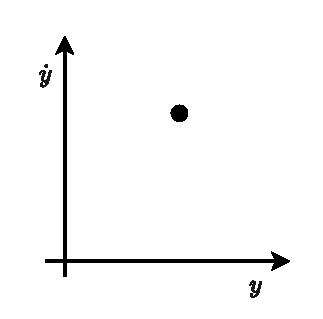
\includegraphics[width=\textwidth]{assets/ex-pianocartesiano}
            \caption{Spazio delle fasi di un punto materiale vincolato a
            muoversi su una retta.}
            \label{fig:ex-pianocartesiano}
        \end{subfigure}
        \hfill
        \begin{subfigure}[t]{0.30\textwidth}
            \centering
            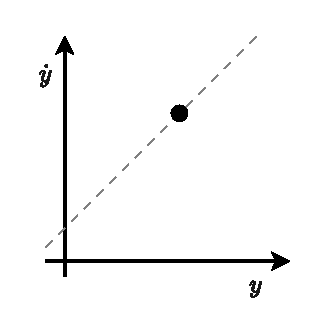
\includegraphics[width=\textwidth]{assets/ex-pianocartesiano-uncontrollable}
            \caption{In base a come è fatta la matrice di controllo $B$, il sistema può
            essere vincolato a muoversi solo su certe traiettorie dello spazio delle fasi.}
            \label{fig:ex-uncontrollable}
        \end{subfigure}
        \hfill
        \begin{subfigure}[t]{0.30\textwidth}
                  \centering
                  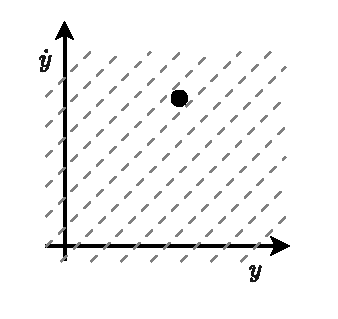
\includegraphics[width=\textwidth]{assets/ex-pianocartesiano-controllable}
                  \caption{Se il sistema è controllabile allora ha accesso a
                  tutti i punti dello spazio delle fasi.}
            \label{fig:ex-controllable}
        \end{subfigure}

        \caption[Punto materiale su una retta]{Esempio di controllabilità di
        un sistema formato da un punto materiale vincolato a muoversi su una retta
        in assenza di forze.}%todo
    \end{figure}


    Sul punto non agiscono forze oltre al controllo $\b u$.
    \label{ex:controllabilità}
\end{example}

\subsection{Scelta degli autovalori}
\label{subsec:scelta-autovalori}
Ho detto nella sezione~\ref{subsec:comportamento-asintotico} che la stabilità
di un sistema lineare è determinata dagli autovalori della matrice associata.
Il concetto di controllabilità di un sistema lineare si traduce nella possibilità
di cambiare gli autovalori associati al sistema in modo arbitrario.
Questo è dovuto al teorema~\ref{thm:eigenvalue-placement} che enuncio di seguito.

\begin{thm}[Scelta degli autovalori]

    Dato un sistema linere
    \begin{equation}
        \dot {\b x} = A\b x + B \b u
        \label{eq:sistema-lineare-controllabile}
    \end{equation}
    dove $A \in \M_{n\times n}(\R)$ e $B \in \M_{n\times m}(\R)$
    e dato un qualsiasi polinomio reale di ordine $n$
    \begin{equation*}
        P(\lambda) = c_1 + \lambda c_2 + \lambda^2 c_3 + \ldots + \lambda^n
    \end{equation*}
    se la matrice di controllabilità $\mathcal C$ del sistema ha rango massimo,
    allora esiste una matrice reale $K$ tale che la matrice
    \begin{equation*}
        A + BK
    \end{equation*}
    ha $P(\lambda)$ come polinomio caratteristico.

    \label{thm:eigenvalue-placement}
\end{thm}

\emph{Dimostrazione}.
Svolgerò la dimostrazione solamente per sistemi in cui $m = 1$, ovvero,
in cui $B$ è un vettore colonna.
La dimostrazione si basa sulla proprietà dei sistemi controllabili di essere
riscritti in una forma detta \emph{forma canonica}:
\begin{equation}
    \tilde A = \left(
        \begin{array}{ccccc}
            0 &1 &0 &\ldots &0 \\
            0 &0 &1 &\ldots &0 \\
            \vdots & & & & \\
            0 &0 &0 &\ldots &1 \\
            -a_1 &-a_2 &-a_3 &\ldots &-a_n
        \end{array}
    \right),\ \tilde B = \left(
    \begin{array}{c}
        0 \\
        0 \\
        \vdots \\
        0 \\
        1
    \end{array}
    \right)
    \label{eq:forma-canonica}
\end{equation}
Per chiarezza, divido la dimostrazione in più passaggi.
\begin{steps}
    \item Mostro che un sistema controllabile può essere riscritto nella forma~\eqref{eq:forma-canonica}.
     Devo trovare una matrice invertibile $T$ tale che
    \begin{equation*}
        T^{-1} A T = \tilde A, \ TB = \tilde B.
    \end{equation*}
    Considero le matrici
    \begin{equation*}
        \mathcal C = (A^{n-1} B, \ldots, AB, B),\
        \tilde {\mathcal C} = (\tilde A^{n-1} \tilde B, \ldots, \tilde A \tilde B, \tilde B),
    \end{equation*}
    entrambe invertibili per ipotesi.
    Voglio dimostrare che prendendo $T = \tilde {\mathcal C} {\mathcal C}^{-1}$ raggiungo l'obiettivo.
    Inizio considerando la matrice $B$. Osservo che
    \begin{equation}
        \mathcal C^{-1}B = (0, \ldots, 0, 1)^{\T} = \tilde B
        \label{eq:c-1b}
    \end{equation}
    in quanto $\mathcal C^{-1} \mathcal C = I$ matrice identità,
    $B$ corrisponde all'ultima colonna di $\mathcal C$ e
    il risultato della~\eqref{eq:c-1b} corrisponde all'ultima riga della matrice identità.
    Vale quindi
    \begin{equation*}
        T B = \tilde {\mathcal C} \mathcal C^{-1} B = \tilde {\mathcal C} \tilde B = \tilde B.
    \end{equation*}

    Ora considero la matrice $A$.
    Vale
    \begin{align*}
        A\mathcal C &= (A^n B, A^{n-1} B, \ldots, AB) \numberthis\label{eq:canb} \\
        &= \left((*), A^{n-1} B, \ldots, AB \right)
    \end{align*}
    dove il termine $(*)$ si ottiene applicando la formula di Cayley-Hamilton
    %todo maybe add citation or source
    al primo termine della~\eqref{eq:canb} e vale
    \begin{equation*}
     (*) = -c_0 B - c_{1} AB \ldots - c_{n-1}A^{n-1} B.
    \end{equation*}
    Ora considero il prodotto delle prime $n-1$ righe di  $\mathcal C^{-1}$
    con le ultime $n-1$ colonne di $A\mathcal C$
    Queste corrispondono alle prime $n-1$ colonne di $\mathcal C$ e il loro prodotto
    con $\mathcal C^{-1}$ da origine a una matrice identità troncata.
    \begin{equation*}
        \mathcal C^{-1} (A^{n-1} B, \ldots, AB) = \left(
        \begin{array}{cccc}
            1 & 0 & \ldots & 0  \\
            0 & 1 & \ldots & 0 \\
            \vdots & & &   \vdots\\
            0 & 0 & \ldots & 1 \\
            0 & 0 & \ldots & 0
        \end{array}
        \right).
    \end{equation*}
    Il termine $(*)$ è un vettore colonna e il suo prodotto con $\mathcal C^{-1}$ vale
    \begin{equation*}
        \mathcal C^{-1}(*) = \left(
             -c_{n-1},
            -c_{n-2},
            \ldots,     -c_0
        \right)^\T.
    \end{equation*}
    Quindi, il prodotto $\mathcal C^{-1}A\mathcal C$ vale
    \begin{equation*}
        \mathcal C^{-1} A \mathcal C = \left(
        \begin{array}{ccccc}
            1 & 0 & \ldots & 0 & c_{n-1} \\
            0 & 1 & \ldots & 0 & c_{n-2}\\
            \vdots & & & &  \vdots\\
            0 & 0 & \ldots & 1 & c_{1}\\
            0 & 0 & \ldots & 0 & c_0
        \end{array}
        \right).
    \end{equation*}
    Per concludere, osservo che il polinomio caratteristico di $A$ e $\tilde A$ è
    lo stesso e quindi trovo lo stesso risultato per $\tilde {\mathcal C}^{-1} \tilde A \tilde C$.
    Trovo quindi che
    \begin{align*}
        \mathcal C^{-1} A\mathcal C &= \tilde {\mathcal C}^{-1} \tilde A \tilde {\mathcal C} \\
        \tilde {\mathcal C}  {\mathcal C}^{-1}A &= \tilde A \tilde {\mathcal C} {\mathcal C}^{-1} \\
        T A &= \tilde A T.
    \end{align*}


    \item Definisco la matrice $K$
    \begin{equation*}
        K = (a_1 - c_1, a_2 - c_2, \ldots, a_n - c_n).
    \end{equation*}
    In questo modo, la matrice $\tilde BK$ è tutta nulla a meno dell'ultima riga, dove
    compaiono i valori di $K$.
    La matrice $\tilde A + \tilde BK$ è quindi
    \begin{equation}
        \tilde A + \tilde BK = \left(
        \begin{array}{ccccc}
            0 &1 &0 &\ldots &0 \\
            0 &0 &1 &\ldots &0 \\
            \vdots & & & &  \vdots\\
            0 &0 &0 &\ldots &1 \\
            c_1 &c_2 &c_3 &\ldots &c_n
        \end{array}
        \right).
        \label{eq:a+bk}
    \end{equation}
    Calcolando il polinomio caratteristico della~\eqref{eq:a+bk}
    usando lo sviluppo di Laplace per le colonne è immediato
    vedere che i suoi coefficienti sono dati proprio dai $c_i$.
\end{steps}
\hfill \qedsymbol \paragraph{}
%todo cite luenberger

Se scelgo come legge di controllo $\b u = K \b x$ e la inserisco
nella~\eqref{eq:sistema-lineare-controllabile}, l'equazione del moto del sistema
diventa
\begin{equation}
    \dot {\b x} = (A + BK) \b x
    \label{eq:controlled-eigenvalues-equation}
\end{equation}
e la matrice $A - BK$ può avere autovalori scelti arbitrariamente.
Nel paragrafo~\ref{sec:controllo-ottimale} illustrerò un criterio per la scelta
degli autovalori di un sistema, al fine di renderlo stabile minimizzando
una funzione costo.


